\documentclass[]{article}
\usepackage{lmodern}
\usepackage{amssymb,amsmath}
\usepackage{ifxetex,ifluatex}
\usepackage{fixltx2e} % provides \textsubscript
\ifnum 0\ifxetex 1\fi\ifluatex 1\fi=0 % if pdftex
  \usepackage[T1]{fontenc}
  \usepackage[utf8]{inputenc}
\else % if luatex or xelatex
  \ifxetex
    \usepackage{mathspec}
  \else
    \usepackage{fontspec}
  \fi
  \defaultfontfeatures{Ligatures=TeX,Scale=MatchLowercase}
\fi
% use upquote if available, for straight quotes in verbatim environments
\IfFileExists{upquote.sty}{\usepackage{upquote}}{}
% use microtype if available
\IfFileExists{microtype.sty}{%
\usepackage{microtype}
\UseMicrotypeSet[protrusion]{basicmath} % disable protrusion for tt fonts
}{}
\usepackage[margin=1in]{geometry}
\usepackage{hyperref}
\hypersetup{unicode=true,
            pdfauthor={; ;},
            pdfborder={0 0 0},
            breaklinks=true}
\urlstyle{same}  % don't use monospace font for urls
\usepackage{color}
\usepackage{fancyvrb}
\newcommand{\VerbBar}{|}
\newcommand{\VERB}{\Verb[commandchars=\\\{\}]}
\DefineVerbatimEnvironment{Highlighting}{Verbatim}{commandchars=\\\{\}}
% Add ',fontsize=\small' for more characters per line
\usepackage{framed}
\definecolor{shadecolor}{RGB}{248,248,248}
\newenvironment{Shaded}{\begin{snugshade}}{\end{snugshade}}
\newcommand{\KeywordTok}[1]{\textcolor[rgb]{0.13,0.29,0.53}{\textbf{#1}}}
\newcommand{\DataTypeTok}[1]{\textcolor[rgb]{0.13,0.29,0.53}{#1}}
\newcommand{\DecValTok}[1]{\textcolor[rgb]{0.00,0.00,0.81}{#1}}
\newcommand{\BaseNTok}[1]{\textcolor[rgb]{0.00,0.00,0.81}{#1}}
\newcommand{\FloatTok}[1]{\textcolor[rgb]{0.00,0.00,0.81}{#1}}
\newcommand{\ConstantTok}[1]{\textcolor[rgb]{0.00,0.00,0.00}{#1}}
\newcommand{\CharTok}[1]{\textcolor[rgb]{0.31,0.60,0.02}{#1}}
\newcommand{\SpecialCharTok}[1]{\textcolor[rgb]{0.00,0.00,0.00}{#1}}
\newcommand{\StringTok}[1]{\textcolor[rgb]{0.31,0.60,0.02}{#1}}
\newcommand{\VerbatimStringTok}[1]{\textcolor[rgb]{0.31,0.60,0.02}{#1}}
\newcommand{\SpecialStringTok}[1]{\textcolor[rgb]{0.31,0.60,0.02}{#1}}
\newcommand{\ImportTok}[1]{#1}
\newcommand{\CommentTok}[1]{\textcolor[rgb]{0.56,0.35,0.01}{\textit{#1}}}
\newcommand{\DocumentationTok}[1]{\textcolor[rgb]{0.56,0.35,0.01}{\textbf{\textit{#1}}}}
\newcommand{\AnnotationTok}[1]{\textcolor[rgb]{0.56,0.35,0.01}{\textbf{\textit{#1}}}}
\newcommand{\CommentVarTok}[1]{\textcolor[rgb]{0.56,0.35,0.01}{\textbf{\textit{#1}}}}
\newcommand{\OtherTok}[1]{\textcolor[rgb]{0.56,0.35,0.01}{#1}}
\newcommand{\FunctionTok}[1]{\textcolor[rgb]{0.00,0.00,0.00}{#1}}
\newcommand{\VariableTok}[1]{\textcolor[rgb]{0.00,0.00,0.00}{#1}}
\newcommand{\ControlFlowTok}[1]{\textcolor[rgb]{0.13,0.29,0.53}{\textbf{#1}}}
\newcommand{\OperatorTok}[1]{\textcolor[rgb]{0.81,0.36,0.00}{\textbf{#1}}}
\newcommand{\BuiltInTok}[1]{#1}
\newcommand{\ExtensionTok}[1]{#1}
\newcommand{\PreprocessorTok}[1]{\textcolor[rgb]{0.56,0.35,0.01}{\textit{#1}}}
\newcommand{\AttributeTok}[1]{\textcolor[rgb]{0.77,0.63,0.00}{#1}}
\newcommand{\RegionMarkerTok}[1]{#1}
\newcommand{\InformationTok}[1]{\textcolor[rgb]{0.56,0.35,0.01}{\textbf{\textit{#1}}}}
\newcommand{\WarningTok}[1]{\textcolor[rgb]{0.56,0.35,0.01}{\textbf{\textit{#1}}}}
\newcommand{\AlertTok}[1]{\textcolor[rgb]{0.94,0.16,0.16}{#1}}
\newcommand{\ErrorTok}[1]{\textcolor[rgb]{0.64,0.00,0.00}{\textbf{#1}}}
\newcommand{\NormalTok}[1]{#1}
\usepackage{graphicx,grffile}
\makeatletter
\def\maxwidth{\ifdim\Gin@nat@width>\linewidth\linewidth\else\Gin@nat@width\fi}
\def\maxheight{\ifdim\Gin@nat@height>\textheight\textheight\else\Gin@nat@height\fi}
\makeatother
% Scale images if necessary, so that they will not overflow the page
% margins by default, and it is still possible to overwrite the defaults
% using explicit options in \includegraphics[width, height, ...]{}
\setkeys{Gin}{width=\maxwidth,height=\maxheight,keepaspectratio}
\IfFileExists{parskip.sty}{%
\usepackage{parskip}
}{% else
\setlength{\parindent}{0pt}
\setlength{\parskip}{6pt plus 2pt minus 1pt}
}
\setlength{\emergencystretch}{3em}  % prevent overfull lines
\providecommand{\tightlist}{%
  \setlength{\itemsep}{0pt}\setlength{\parskip}{0pt}}
\setcounter{secnumdepth}{0}
% Redefines (sub)paragraphs to behave more like sections
\ifx\paragraph\undefined\else
\let\oldparagraph\paragraph
\renewcommand{\paragraph}[1]{\oldparagraph{#1}\mbox{}}
\fi
\ifx\subparagraph\undefined\else
\let\oldsubparagraph\subparagraph
\renewcommand{\subparagraph}[1]{\oldsubparagraph{#1}\mbox{}}
\fi

%%% Use protect on footnotes to avoid problems with footnotes in titles
\let\rmarkdownfootnote\footnote%
\def\footnote{\protect\rmarkdownfootnote}

%%% Change title format to be more compact
\usepackage{titling}

% Create subtitle command for use in maketitle
\newcommand{\subtitle}[1]{
  \posttitle{
    \begin{center}\large#1\end{center}
    }
}

\setlength{\droptitle}{-2em}
  \title{\bf{Project B Report}}
  \pretitle{\vspace{\droptitle}\centering\huge}
  \posttitle{\par}
\subtitle{STAT 331, Fall 2017}
  \author{\text{Rosie Zou (20588049)} \\ \text{Simon Guo (20600133)} \\ \text{Azoacha Forcheh (20558994)}}
  \preauthor{\centering\large\emph}
  \postauthor{\par}
  \date{}
  \predate{}\postdate{}

\usepackage{booktabs}
\usepackage{longtable}
\usepackage{array}
\usepackage{multirow}
\usepackage[table]{xcolor}
\usepackage{wrapfig}
\usepackage{float}
\usepackage{colortbl}
\usepackage{pdflscape}
\usepackage{tabu}
\usepackage{threeparttable}

\usepackage{graphicx}
\usepackage{caption}
\usepackage{subcaption}
\usepackage{float}

\begin{document}
\maketitle

\begin{section}{Summary}
The objective of this report is to model the Apple Stock return rate, defined as $ret.AAPL_i = \frac{AAPL_i - AAPL_{i-1}}{AAPL_{i-1}}$, based on key metrics such as volatility, $S\&P$ 500 Index, and etc. 

To model the return rate, our group has surveyed a wide range of models including an autoregressive model, linear models from automated model selection, as well as transformed linear models. 

From the autoregressive model, we noticed the heteroscedascity caused by autocorrelation, which led us to determine that directly modelling the stock price is not the most ideal way to model the return rate. We also found discrepancy between the adjusted R-Squared value and the residual plots in the backfitted model, which will be further discussed later in this report. Through our investigation, our group has concluded that there is no truly ideal linear model for the Apple Stock return rate. Nevertheless, we were able to identify the inadequate models and gain insights on why those models did not work.
\end{section}

\begin{section}{Model Selection}
The first model to be considered is the autoregressive model, which directly models the stock price of day $i$ using the price from day $i-1$ and has the following expression: $$ AAPL_i = \beta_0 + \beta_1 AAPL_{i-1}$$

The residual plot from the fitted model has a clearly heteroscedastic property, since the residuals take on a fan shape.

\begin{center}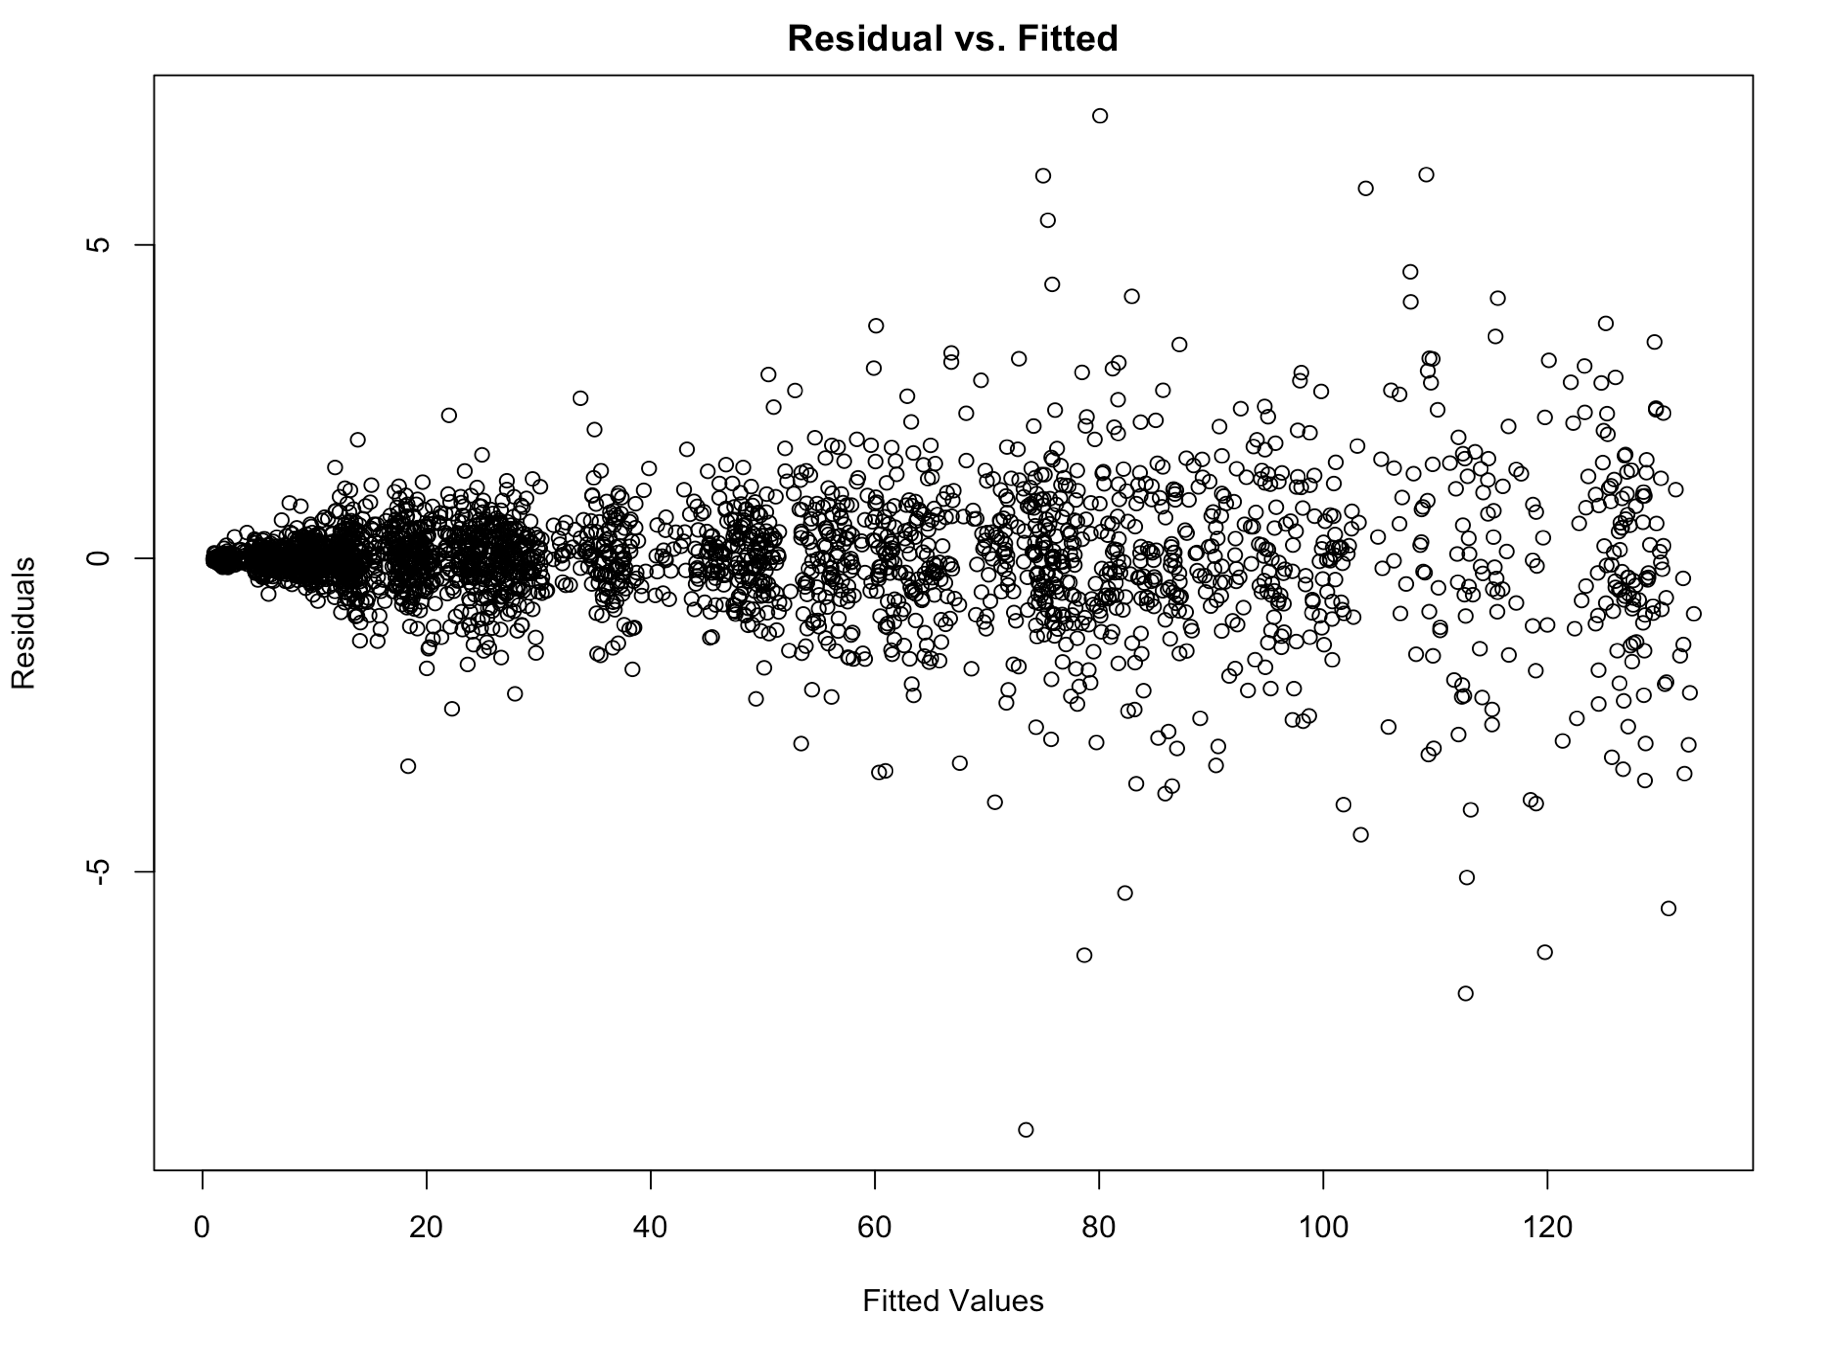
\includegraphics[width=90mm]{autoregressive_residual_vs_fitted.png}\end{center}

We tried to resolve the heteroscedascity issue by implementing a Weighted Least Squares autoregressive model but the results remained the same (see Appendix for full code and plot comparison). After some research, it turns out that this is an irreducible property of the autoregressive model because the data is serially correlated. We realized that we needed something better than directly modelling the price. Hence we decided to directly model the return which, to re-iterate, is defined as $ret.AAPL_i = \frac{AAPL_i - AAPL_{i-1}}{AAPL_{i-1}}$.

Correlation between the coefficients was also expected from the data. Since it is a time-series financial data set, we knew and verified that time is correlated to variables such as the Apple Stock Price and the $S \& P$ 500 Index. The detailed matrix can be found in the Appendix section. We decided that this wasn't too much of an issue since it is an inevitable part of any time-series data.

Moving on from the autoregressive model, we then considered automated model selecting using forward selection, backward elemination, and stepwise selection, from which we obtained the following models (full code in Appendix):


\textbf{Forward selection: } $Return = \beta_0 + \beta_1VIX + \beta_2AAPL2 + \beta_3AAPL + \beta_4SPGSCITR$

\textbf{Backward elimination: } $Return = \beta_0 + \beta_1AAPL + \beta_2VIX + \beta_3SPGSCITR + \beta_4AAPL2$

\textbf{Stepwise selection: } $Return = \beta_0 + \beta_1VIX + \beta_2AAPL2 + \beta_3AAPL + \beta_4SPGSCITR$


Interestingly, all selection methods returned the same model. Before we proceeded any further, we consulted with Prof. Zeng. After receiving helpful advice from the professor, we realized that since $Return$ is calculated as a function of $AAPL$ and $AAPL2$, the two variables cannot be included in the same model. We then adjusted the full model by excluding the variable $AAPL$, hence only keeping the previous-day price, and obtained the results below:


\textbf{Forward selection: } $ Return = \beta_0 + \beta_1VIX + \beta_2AAPL2 + \beta_3SPGSCITR + \beta_4EEM$

\textbf{Backward elimination: } $ Return = \beta_0 + \beta_1VIX + \beta_2AAPL2 + \beta_3SPGSCITR + \beta_4EEM$

\textbf{Stepwise selection: } $ Return = \beta_0 + \beta_1VIX + \beta_2AAPL2 + \beta_3SPGSCITR + \beta_4EEM$

We decided to further analyze this model in the model diagnostics section.

Additionally, we considered how the distribution of the independent variables could affect the model fit. Since both $VIX$ and $SPGSCITR$ had heavily skewed histograms, we decided to log-transform the variables to make the distributions resemble a normal curve and obtained the following model:
\textbf{Transformed model: } $ Return = \beta_0 + \beta_1(log(VIX)^{-2}) + \beta_2AAPL2 + \beta_3(log(SPGSCITR)) + \beta_4EEM$. This will be the second model to be discussed in the model diagnostics section.

\end{section}

\begin{section}{Model Diagnostics}

We first look into some diagnostic plots of the two models for the sake of residual analysis and outlier detection.

\begin{figure}[H]
\begin{subfigure}{.5\textwidth}
  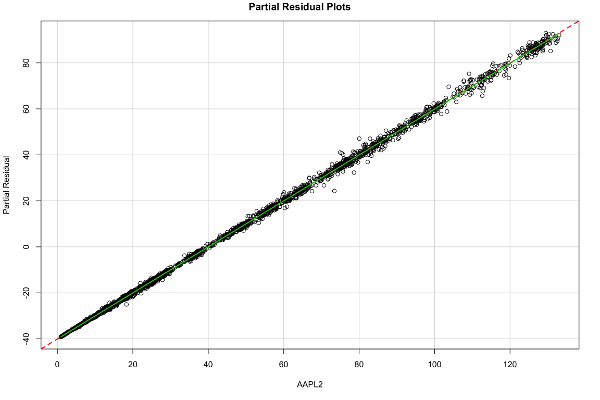
\includegraphics[width=85mm]{diagnostics/arm_covar_residuals.png}
  \caption{Autoregressive Model}
\end{subfigure}%
\begin{subfigure}{.5\textwidth}
  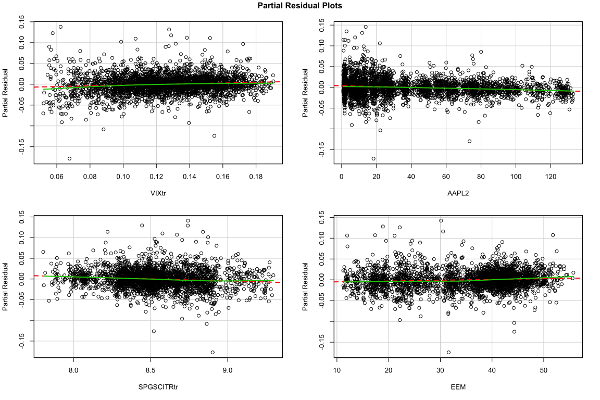
\includegraphics[width=85mm]{diagnostics/fm_covar_residuals.png}
  \caption{Automated Model}
\end{subfigure}
\end{figure}

There is a strong linear trend in the partial residual plot of the autoregressive model, and no deviation from the straight line. We see this trend with the covariates of the automated model as well, with only the `EEM` covariate and the log-transformed `VIX` displaying a small amount of deviation from the straight line. Hence, the assumption of linearity is satisfied for both models.

The residuals of the autoregressive model are heteroscedastic as the plot of the residuals versus the fitted values has a fan-shaped pattern. In addition, the Q-Q plot of the residuals is heavy-tailed and exhibits curvature. In comparison, the plot of the residuals versus the fitted values of the automated model has more randomness and lacks the fan-shaped pattern indicative of heteroscedasticity; the Q-Q plot, while still being heavy-tailed, follows the linear trend more closely. 

\begin{figure}[H]
\begin{subfigure}{.5\textwidth}
  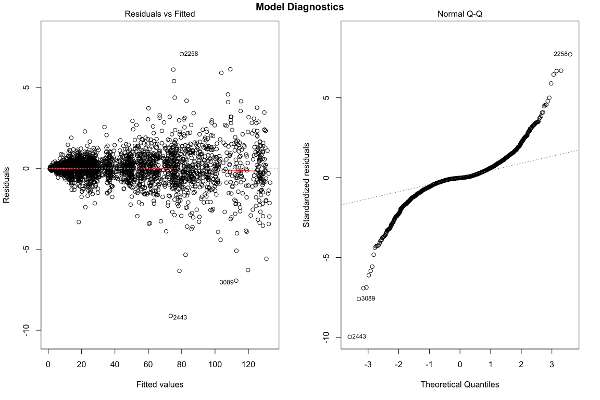
\includegraphics[width=85mm]{diagnostics/arm_model_plots.png}
  \caption{Autoregressive Model}
\end{subfigure}%
\begin{subfigure}{.5\textwidth}
  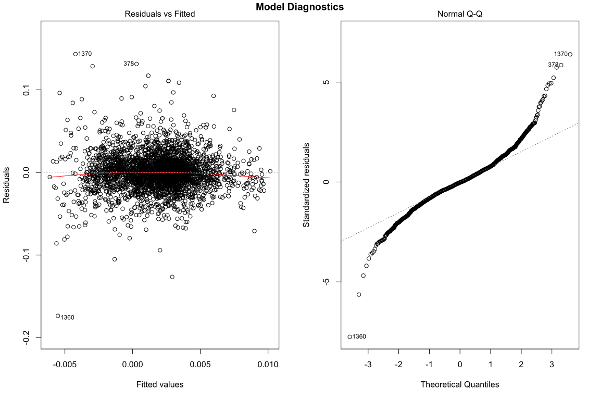
\includegraphics[width=85mm]{diagnostics/fm_model_plots.png}
  \caption{Automated Model}
\end{subfigure}
\end{figure}

Hence, the automated model produces errors that satisfy the assumption of constant error variance and that have non-normality that might be reasonably ignored, while the plots of the autoregressive model indicate that there are non-constant variances of the error and non-normality that we may be able to fix.


\begin{figure}[H]
\begin{subfigure}{.5\textwidth}
  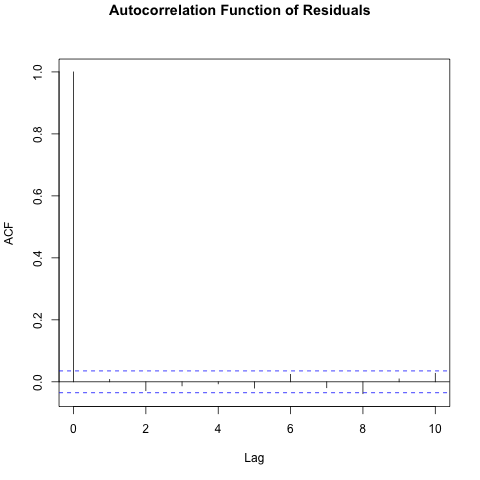
\includegraphics[width=85mm]{diagnostics/arm_acf_residuals.png}
  \caption{Autoregressive Model}
\end{subfigure}%
\begin{subfigure}{.5\textwidth}
  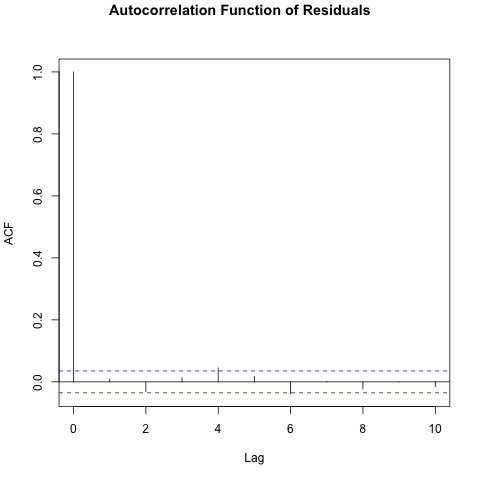
\includegraphics[width=85mm]{diagnostics/fm_acf_residuals.png}
  \caption{Automated Model}
\end{subfigure}
\end{figure}

We then looked into the last assumption of linear regression models: independence of the errors. As the stock data was time-series data and contained serial correlation, a scatterplot matrix was ruled out as a useful tool for detecting correlation. We instead considered ACF plots of the residuals, in combination with the results of the Durbin-Watson test. As can be seen in the ACF plots above, both models have explained away the autocorrelation in the residuals very well, as almost all of the sample correlations are within the limits. The results of the Durbin-Watson test on the models (shown in the table below) confirms this: for both models, the $p$-value of the test is high enough to accept the null hypothesis that there is no autocorrelation between the residuals.




\begin{table}[H]
\centering
\begin{tabular}{l|r|r}
\hline
  & Test Statistic & p-value\\
\hline
Autoregressive & 1.989882 & 0.7398676\\
\hline
Automated & 1.992961 & 0.8450008\\
\hline
\multicolumn{3}{l}{\textsuperscript{*} alternative: true autocorrelation is not}\\
\multicolumn{3}{l}{0}\\
\end{tabular}
\end{table}

The next concern we addressed was potential outliers and high-leverage cases. In both Cook's Distance plots below, there are no concerning observations that have a distance greater than 1, but most observations have a Cook's Distance greater than $\frac{p}{n}$, which is 0.001612 and 0.000403 for the automated and the autoregressive model, respectively. However, we see in both Residuals versus Leverage plots that there are no cases that are influential to the regression results. All points are well enough within the Cook's distance lines that said lines do not appear on either plot.

\begin{figure}[H]
\begin{subfigure}{.5\textwidth}
  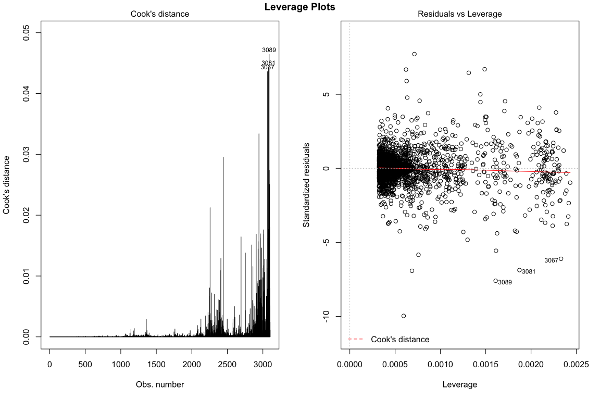
\includegraphics[width=85mm]{diagnostics/arm_leverage_plots.png}
  \caption{Autoregressive Model}
\end{subfigure}%
\begin{subfigure}{.5\textwidth}
  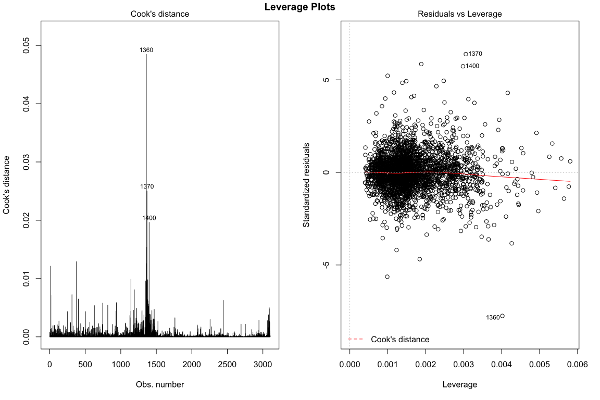
\includegraphics[width=85mm]{diagnostics/fm_leverage_plots.png}
  \caption{Automated Model}
\end{subfigure}
\end{figure}



Once we had performed residual analysis and outlier detection, we performed cross validation for the two models to determine if they were overfitting. The $k$-fold cross validation method was used - with $k=10$ - and the $RMSE$ over the 10 folds was calculated. For the sake of comparison, since the models have different dependent variables and hence different scales, the $RMSE$ had to be normalized by dividing it by the range of the observed values. We denote this calculation as the $NRMSE$. 

The autoregressive model has an $NRMSE$ of 0.0071775, a value very close to 0, indicating that this model is a very good fit. While still being a well-fitted model, the automated model will generally produce less accurate predictions than the former model as it has a higher $NRMSE$ of 0.0706321.

We explored this claim by using the two models to predict responses for a test set of data, obtained by splitting the original dataset via an 80:20 split. The plots below are of the distributions of the error of prediction obtained from this test.

\begin{figure}[H]
  \centering
  \includegraphics[width=85mm]{diagnostics/prediction_histograms.png}
  \captionsetup{labelformat=empty}
  \caption{Prediction Error Histograms}
\end{figure}

The autoregressive model produces far more inaccurate results when predicting, with the value of the residual being as high as 6 in some cases. The autoselected model performs extremely well, producing a higher number of accurate predictions and a much smaller range of error.

Based on our aforementioned results, the final model we decided to choose was the automated model, i.e. $ Return = \beta_0 + \beta_1(log(VIX)^{-2}) + \beta_2AAPL2 + \beta_3(log(SPGSCITR)) + \beta_4EEM$. While both models are well-fitted with most of the linear regression assumptions satisified and no significant outliers, the residuals of the automated model are homoscedastic and are closer to normality than those of the autoregressive model. In addition, though the autoregressive model is less overfitted than the automated model (as measured by the $NRMSE$), it is not by a significant difference and the automated model tends to produces more accurate predictions. 

The paramters estimates and confidence interval of the final model are displayed in the table below.

\begin{table}[H]
\centering
\begin{tabular}{l|r|l}
\hline
  & Estimate & Intervals\\
\hline
(Intercept) & 0.0729816 & [0.0311, 0.1149]\\
\hline
VIXtr & 0.0829201 & [0.047, 0.1189]\\
\hline
AAPL2 & -0.0000878 & [-1e-04, 0]\\
\hline
SPGSCITRtr & -0.0098632 & [-0.0151, -0.0046]\\
\hline
EEM & 0.0001745 & [0, 3e-04]\\
\hline
\end{tabular}
\end{table}

We conclude that neither model is a good enough fit. However, while the automated model has a low Adjusted $R^2$, it predicts very accurately and is a strong model otherwise. Given more time and resources, we could potentially develop a better model using the knowledge we now have about the relationship between the covariates and the response. 

For example, an artificial neural net could be implemented instead, especially as this is a popular method for predicting stock returns and there is more research that can be considered during implementation. Alternatively, we could build on the autoregressive model to create an ARIMA model, which a good choice of model for time series data such as this.

\end{section}

\begin{section}{Discussion}

We answer the questions posed to us in the Instructions file in this section.

\begin{enumerate}
\item{}
\textit {What are the most important factors affecting Apple Stock returns?}

According to the results from the R code below, we can check the $p$-values for the significance of coefficients with the corresponding covariates. For the transformed model, $VIX$ term has the lowest $p$-value as shown in the summary, which means it would make largest change to the response if it drops out of the model; while $AAPL2$ term, which is the pervious day's price, and $SPGSCITR$ term's coefficients ealso have relatively small $p$-values. For our selected model before transformation, $VIX$ has the lowest p-value as well, and again $AAPL2$ and $SPGSCITR$ terms' coefficients have considerably small $p$-values too.  So based on our models, $VIX$ would be the most important factor, and $SPGSCITR$ and $AAPL2$ are considerably significant as well. 

\item{}
\textit {Does including information for several days ago have much of an impact on tomorrow’s return, if we account for today’s information?}

As shown in the R code in the Appendix, after attempting to instead of using previous day's price to calculate return, we take the average of the previous 5 days' stock prices and still fitting the same transformed model. Comparing to original transformed model, the performance of the model seems to be better in temrs of coefficient of determination and the AIC values, while there is a small increase in adjusted $R^2$ and a small decrease for AIC. So it seems that from our attempt, including information for several days ago would give a better model fitting the tomorrow's return, while we are still accounting for today's information.

\item{}
\textit {Does the model predict accurately?}

Based on our results on our k-fold cross validation with the comparsion of training and testing sets of data, the model performs generally well for prediction accuracy. Although in the summary of the model, the coefficient of determination is not ideally high, as we have discussed in class and the fact that $R^2$ can be affected by other factors (such as number of variables that are involved), so it would be acceptable to say that the model predicts the future value with reasonably accurate results. 

\item{}
\textit {Are there any coefficients with high $p$-values retained in the final model? If so, why?}

According our models, fortunately we don't have any coefficients with high $p$-values retained in the final model. All of the coefficients have descent $p$-values that are lower than 0.05.

\item{}
\textit {Are any of the regression assumptions of the final model violated? If so, which ones?}

This question has been mentioned along with the Model Diagnostics part. All of the regression assumptions seems to be satisfied by our final model, instead of there is a little bit bias on the independence of residuals.

\item{}
\textit {What are the possible deficiencies of the final model? How the model can be improved?}

As discussed in previous analysis part, and also by looking at the residual plots and the summary of aborted models, the data has a tendency to be fitting a non-linear model. For example, there is a curved trend for the residual against fitted values plot, even after the chosen transformation. And notice that from the R results we can see that the adjusted and unadjusted coefficients of determination is very small and not close to 1 at all, which is not ideal as well. To improve the fittness of the model, it might make more sense to fit a non-linear model instead. Alternatively, there is the option of adding more covariates to the model, but that would increase the possiblity of overfitting the model.  

\item{}
\textit {Are there any outlying observations that might be appropriate to remove?}

By judging from the results of residual plots and leverage plots, it can be seen that there seems to have several outliers concentrated around the year 2008, which has the index 1370. The possible reason for the outlying results could be the finacial crisis during that time that would cause the drop in variates' values, but AAPL stock price didn't be affected that much, possible explanation could be the release of new series of iPhone which sort of stablize the change in stock price for Apple. Under such circumstance, there might exist possible reasons for the unexpected change, here it would be more reasonable to ignore the outlying results, as it is not really "unexpected" or it is abnormal. Therefore, it would not be appropriate to remove these values.

\end{enumerate}

\end{section}

\newpage

\begin{section}{Appendix}
Below is a collection of R code used in this report.
\end{section}

\subsubsection{Pre-process the data}\label{pre-process-the-data}

\begin{Shaded}
\begin{Highlighting}[]
\NormalTok{market_origin <-}\StringTok{ }\KeywordTok{read.csv}\NormalTok{(}\StringTok{"market_index_clean.csv"}\NormalTok{)}
\NormalTok{first <-}\StringTok{ }\NormalTok{market_origin[}\DecValTok{1}\NormalTok{,]}
\NormalTok{market <-}\StringTok{ }\NormalTok{market_origin[}\DecValTok{2}\OperatorTok{:}\DecValTok{3104}\NormalTok{,]}
\NormalTok{market}\OperatorTok{$}\NormalTok{AAPL2 <-}\StringTok{ }\NormalTok{market_origin[,}\StringTok{"AAPL"}\NormalTok{][}\DecValTok{1}\OperatorTok{:}\DecValTok{3103}\NormalTok{]}
\NormalTok{market}\OperatorTok{$}\NormalTok{Return <-}\StringTok{ }\NormalTok{(market}\OperatorTok{$}\NormalTok{AAPL }\OperatorTok{-}\StringTok{ }\NormalTok{market}\OperatorTok{$}\NormalTok{AAPL2)}\OperatorTok{/}\NormalTok{market}\OperatorTok{$}\NormalTok{AAPL2}

\NormalTok{market}\OperatorTok{$}\NormalTok{Date <-}\StringTok{ }\NormalTok{market_origin}\OperatorTok{$}\NormalTok{Date[}\DecValTok{2}\OperatorTok{:}\DecValTok{3104}\NormalTok{]}
\NormalTok{date <-}\StringTok{ }\NormalTok{market}\OperatorTok{$}\NormalTok{Date}
\NormalTok{first <-}\StringTok{ }\NormalTok{date[}\DecValTok{1}\NormalTok{]}
\NormalTok{day <-}\StringTok{ }\KeywordTok{c}\NormalTok{()}
\ControlFlowTok{for}\NormalTok{(i }\ControlFlowTok{in} \DecValTok{1}\OperatorTok{:}\KeywordTok{length}\NormalTok{(date)) \{}
\NormalTok{  diff =}\StringTok{ }\KeywordTok{round}\NormalTok{(}\KeywordTok{difftime}\NormalTok{(date[i], first))}
\NormalTok{  day =}\StringTok{ }\KeywordTok{c}\NormalTok{(day, diff)}
\NormalTok{\}}
\NormalTok{market}\OperatorTok{$}\NormalTok{Date <-}\StringTok{ }\NormalTok{day}

\NormalTok{## Splitting the data into a training and test set (80/20)}
\NormalTok{n <-}\StringTok{ }\KeywordTok{length}\NormalTok{(market[,}\DecValTok{1}\NormalTok{])}
\NormalTok{split <-}\StringTok{ }\KeywordTok{round}\NormalTok{(}\FloatTok{0.8}\OperatorTok{*}\NormalTok{n)}
\NormalTok{market_train <-}\StringTok{ }\NormalTok{market[}\DecValTok{1}\OperatorTok{:}\NormalTok{split,]}
\NormalTok{market_test <-}\StringTok{ }\NormalTok{market[(split}\OperatorTok{+}\DecValTok{1}\NormalTok{)}\OperatorTok{:}\NormalTok{n,]}
\end{Highlighting}
\end{Shaded}

\subsubsection{Full Model}\label{full-model}

\begin{Shaded}
\begin{Highlighting}[]
\NormalTok{full_model <-}\StringTok{ }\KeywordTok{lm}\NormalTok{(Return}\OperatorTok{~}\NormalTok{., }\DataTypeTok{data =}\NormalTok{ market)}
\KeywordTok{summary}\NormalTok{(full_model)}
\end{Highlighting}
\end{Shaded}

\subsubsection{Null Model}\label{null-model}

\begin{Shaded}
\begin{Highlighting}[]
\NormalTok{null_model <-}\StringTok{ }\KeywordTok{lm}\NormalTok{(Return}\OperatorTok{~}\DecValTok{1}\NormalTok{, }\DataTypeTok{data =}\NormalTok{ market)}
\KeywordTok{summary}\NormalTok{(null_model)}
\end{Highlighting}
\end{Shaded}

\subsubsection{Autoregressive Model}\label{autoregressive-model}

\begin{Shaded}
\begin{Highlighting}[]
\NormalTok{autoregressive_model <-}\StringTok{ }\KeywordTok{lm}\NormalTok{(AAPL}\OperatorTok{~}\NormalTok{AAPL2, }\DataTypeTok{data =}\NormalTok{ market_train)}
\KeywordTok{plot}\NormalTok{(}\KeywordTok{fitted}\NormalTok{(autoregressive_model),}\KeywordTok{residuals}\NormalTok{(autoregressive_model), }
     \DataTypeTok{main =} \StringTok{"Residual vs. Fitted"}\NormalTok{, }\DataTypeTok{xlab =} \StringTok{"Fitted Values"}\NormalTok{, }\DataTypeTok{ylab =} \StringTok{"Residuals"}\NormalTok{)}
\end{Highlighting}
\end{Shaded}

\subsubsection{WLS Autoregressive Model}\label{wls-autoregressive-model}

\begin{Shaded}
\begin{Highlighting}[]
\NormalTok{wts <-}\DecValTok{1}\OperatorTok{/}\NormalTok{(}\KeywordTok{fitted}\NormalTok{(}\KeywordTok{lm}\NormalTok{(}\KeywordTok{abs}\NormalTok{(}\KeywordTok{residuals}\NormalTok{(autoregressive_model))}\OperatorTok{~}\KeywordTok{fitted}\NormalTok{(autoregressive_model)))}\OperatorTok{^}\DecValTok{2}\NormalTok{)}
\NormalTok{wls <-}\StringTok{ }\KeywordTok{lm}\NormalTok{(market_train}\OperatorTok{$}\NormalTok{AAPL}\OperatorTok{~}\NormalTok{market}\OperatorTok{$}\NormalTok{AAPL2, }\DataTypeTok{weights =}\NormalTok{ wts)}
\KeywordTok{par}\NormalTok{(}\DataTypeTok{mfrow=}\KeywordTok{c}\NormalTok{(}\DecValTok{1}\NormalTok{,}\DecValTok{2}\NormalTok{))}
\KeywordTok{plot}\NormalTok{(}\KeywordTok{fitted}\NormalTok{(autoregressive_model), autoregressive_model}\OperatorTok{$}\NormalTok{residuals, }
     \DataTypeTok{main=}\StringTok{"unweighted"}\NormalTok{, }\DataTypeTok{xlab =} \StringTok{"fitted"}\NormalTok{, }\DataTypeTok{ylab =} \StringTok{"residuals"}\NormalTok{)}
\KeywordTok{plot}\NormalTok{(}\KeywordTok{fitted}\NormalTok{(wls), wls}\OperatorTok{$}\NormalTok{residuals, }\DataTypeTok{main=}\StringTok{"weighted"}\NormalTok{, }\DataTypeTok{xlab =} \StringTok{"fitted"}\NormalTok{, }\DataTypeTok{ylab =} \StringTok{"residuals"}\NormalTok{)}
\end{Highlighting}
\end{Shaded}

There is no apparent difference between the weighted least squares and
the un-weighted autoregressive models.

\subsubsection{Correlation Matrix}\label{correlation-matrix}

\begin{Shaded}
\begin{Highlighting}[]
\KeywordTok{cor}\NormalTok{(market_train)}
\end{Highlighting}
\end{Shaded}

\subsubsection{Forward Selection}\label{forward-selection}

\begin{Shaded}
\begin{Highlighting}[]
\KeywordTok{step}\NormalTok{(null_model, }\DataTypeTok{scope =} \KeywordTok{list}\NormalTok{(}\DataTypeTok{upper=}\NormalTok{full_model), }\DataTypeTok{direction=}\StringTok{"forward"}\NormalTok{)}
\KeywordTok{summary}\NormalTok{(}\KeywordTok{lm}\NormalTok{(}\DataTypeTok{formula =}\NormalTok{ Return }\OperatorTok{~}\StringTok{ }\NormalTok{VIX }\OperatorTok{+}\StringTok{ }\NormalTok{AAPL2 }\OperatorTok{+}\StringTok{ }\NormalTok{AAPL }\OperatorTok{+}\StringTok{ }\NormalTok{SPGSCITR, }\DataTypeTok{data =}\NormalTok{ market_train))}
\end{Highlighting}
\end{Shaded}

\subsubsection{Backward Elimination}\label{backward-elimination}

\begin{Shaded}
\begin{Highlighting}[]
\KeywordTok{step}\NormalTok{(full_model, }\DataTypeTok{scope =} \KeywordTok{list}\NormalTok{(}\DataTypeTok{lower=}\NormalTok{null_model), }\DataTypeTok{direction=}\StringTok{"backward"}\NormalTok{)}
\KeywordTok{summary}\NormalTok{(}\KeywordTok{lm}\NormalTok{(}\DataTypeTok{formula =}\NormalTok{ Return }\OperatorTok{~}\StringTok{ }\NormalTok{AAPL }\OperatorTok{+}\StringTok{ }\NormalTok{VIX }\OperatorTok{+}\StringTok{ }\NormalTok{SPGSCITR }\OperatorTok{+}\StringTok{ }\NormalTok{AAPL2, }\DataTypeTok{data =}\NormalTok{ market_train))}
\end{Highlighting}
\end{Shaded}

\subsubsection{Stepwise Selection}\label{stepwise-selection}

\begin{Shaded}
\begin{Highlighting}[]
\KeywordTok{step}\NormalTok{(null_model, }\DataTypeTok{scope =} \KeywordTok{list}\NormalTok{(}\DataTypeTok{upper=}\NormalTok{full_model), }\DataTypeTok{direction=}\StringTok{"both"}\NormalTok{)}
\end{Highlighting}
\end{Shaded}

\subsubsection{Forward Selection without
AAPL}\label{forward-selection-without-aapl}

\begin{Shaded}
\begin{Highlighting}[]
\NormalTok{full_model <-}\StringTok{ }\KeywordTok{lm}\NormalTok{(Return}\OperatorTok{~}\NormalTok{SPX}\OperatorTok{+}\NormalTok{VIX}\OperatorTok{+}\NormalTok{SPGSCITR}\OperatorTok{+}\NormalTok{BNDGLB}\OperatorTok{+}\NormalTok{EEM}\OperatorTok{+}\NormalTok{AAPL2, }\DataTypeTok{data =}\NormalTok{ market)}
\KeywordTok{step}\NormalTok{(null_model, }\DataTypeTok{scope =} \KeywordTok{list}\NormalTok{(}\DataTypeTok{upper=}\NormalTok{full_model), }\DataTypeTok{direction=}\StringTok{"forward"}\NormalTok{)}
\end{Highlighting}
\end{Shaded}

\subsubsection{Backward Elimination without
AAPL}\label{backward-elimination-without-aapl}

\begin{Shaded}
\begin{Highlighting}[]
\KeywordTok{step}\NormalTok{(full_model, }\DataTypeTok{scope =} \KeywordTok{list}\NormalTok{(}\DataTypeTok{lower=}\NormalTok{null_model), }\DataTypeTok{direction=}\StringTok{"backward"}\NormalTok{)}
\end{Highlighting}
\end{Shaded}

\subsubsection{Stepwise Selection without
AAPL}\label{stepwise-selection-without-aapl}

\begin{Shaded}
\begin{Highlighting}[]
\KeywordTok{step}\NormalTok{(null_model, }\DataTypeTok{scope =} \KeywordTok{list}\NormalTok{(}\DataTypeTok{upper=}\NormalTok{full_model), }\DataTypeTok{direction=}\StringTok{"both"}\NormalTok{)}
\end{Highlighting}
\end{Shaded}

\subsubsection{Log-transformed model from stepwise selection
results}\label{log-transformed-model-from-stepwise-selection-results}

\begin{Shaded}
\begin{Highlighting}[]
\NormalTok{## note that the VIX needed to be raised to the -2, after the log transformation}
\NormalTok{##  in order to obtain a distribution close to the Gaussian curve}
\NormalTok{market.tr <-}\StringTok{ }\NormalTok{market}
\NormalTok{market.tr}\OperatorTok{$}\NormalTok{VIXtr <-}\StringTok{ }\KeywordTok{log}\NormalTok{(market}\OperatorTok{$}\NormalTok{VIX)}\OperatorTok{^}\NormalTok{(}\OperatorTok{-}\DecValTok{2}\NormalTok{)}
\NormalTok{market.tr}\OperatorTok{$}\NormalTok{SPGSCITRtr <-}\StringTok{ }\KeywordTok{log}\NormalTok{(market}\OperatorTok{$}\NormalTok{SPGSCITR)}
\NormalTok{market.tr_train <-}\StringTok{ }\NormalTok{market.tr[}\DecValTok{1}\OperatorTok{:}\NormalTok{split,]}
\NormalTok{market.tr_test <-}\StringTok{ }\NormalTok{market.tr[(split}\OperatorTok{+}\DecValTok{1}\NormalTok{)}\OperatorTok{:}\NormalTok{n,]}

\NormalTok{transformed_model <-}\StringTok{ }\KeywordTok{lm}\NormalTok{(Return}\OperatorTok{~}\NormalTok{VIXtr}\OperatorTok{+}\NormalTok{AAPL2}\OperatorTok{+}\NormalTok{SPGSCITRtr}\OperatorTok{+}\NormalTok{EEM, }\DataTypeTok{data=}\NormalTok{market.tr_train)}
\KeywordTok{summary}\NormalTok{(transformed_model)}
\end{Highlighting}
\end{Shaded}

\subsubsection{Function for plotting diagnostic
tools}\label{function-for-plotting-diagnostic-tools}

\begin{Shaded}
\begin{Highlighting}[]
\NormalTok{diagnostic_plots <-}\StringTok{ }\ControlFlowTok{function}\NormalTok{(model) \{}
\NormalTok{  p <-}\StringTok{ }\KeywordTok{length}\NormalTok{(model}\OperatorTok{$}\NormalTok{coef) }\OperatorTok{-}\StringTok{ }\DecValTok{1} \CommentTok{# the number of covariates in the model}
\NormalTok{  nrows <-}\StringTok{ }\NormalTok{p}\OperatorTok\DecValTok{2}
\NormalTok{  savepar <-}\StringTok{ }\KeywordTok{par}\NormalTok{(}\DataTypeTok{mfrow=}\KeywordTok{c}\NormalTok{(}\DecValTok{1}\NormalTok{,}\DecValTok{1}\NormalTok{))}
  \ControlFlowTok{if}\NormalTok{ (nrows }\OperatorTok{>}\StringTok{ }\DecValTok{0}\NormalTok{) \{}
\NormalTok{    savepar <-}\StringTok{ }\KeywordTok{par}\NormalTok{(}\DataTypeTok{mfrow=}\KeywordTok{c}\NormalTok{(nrows, }\DecValTok{2}\NormalTok{))}
\NormalTok{  \}}
  
  \CommentTok{# Partial Residual v.s. Covariates Plot}
\NormalTok{  savepar}
  \KeywordTok{crPlots}\NormalTok{(model, }\DataTypeTok{ylab=}\StringTok{"Partial Residual"}\NormalTok{, }\DataTypeTok{smooth=}\NormalTok{T,}
          \DataTypeTok{main=}\StringTok{''}\NormalTok{)}
  \KeywordTok{title}\NormalTok{(}\StringTok{"Partial Residual Plots"}\NormalTok{, }
        \DataTypeTok{outer=}\NormalTok{T, }\DataTypeTok{line=}\OperatorTok{-}\DecValTok{1}\NormalTok{)}
  
  \CommentTok{# Q-Q Plot and Residual v.s. Fitted Plot }
  \KeywordTok{par}\NormalTok{(}\DataTypeTok{mfrow=}\KeywordTok{c}\NormalTok{(}\DecValTok{1}\NormalTok{,}\DecValTok{2}\NormalTok{))}
  \KeywordTok{plot}\NormalTok{(model, }\DataTypeTok{which=}\KeywordTok{c}\NormalTok{(}\DecValTok{1}\NormalTok{,}\DecValTok{2}\NormalTok{))}
  \KeywordTok{title}\NormalTok{(}\KeywordTok{paste}\NormalTok{(}\StringTok{"Model Diagnostics"}\NormalTok{),}
        \DataTypeTok{outer=}\NormalTok{T, }\DataTypeTok{line=}\OperatorTok{-}\DecValTok{1}\NormalTok{)}
  
\NormalTok{  ## Leverage Plots}
  \KeywordTok{par}\NormalTok{(}\DataTypeTok{mfrow=}\KeywordTok{c}\NormalTok{(}\DecValTok{1}\NormalTok{,}\DecValTok{2}\NormalTok{))}
  \KeywordTok{plot}\NormalTok{(model, }\DataTypeTok{which=}\KeywordTok{c}\NormalTok{(}\DecValTok{4}\NormalTok{,}\DecValTok{5}\NormalTok{))}
  \KeywordTok{title}\NormalTok{(}\KeywordTok{paste}\NormalTok{(}\StringTok{"Leverage Plots"}\NormalTok{),}
        \DataTypeTok{outer=}\NormalTok{T, }\DataTypeTok{line=}\OperatorTok{-}\DecValTok{1}\NormalTok{)}
\NormalTok{\}}

\KeywordTok{diagnostic_plots}\NormalTok{(autoregressive_model)}
\KeywordTok{diagnostic_plots}\NormalTok{(transformed_model)}
\end{Highlighting}
\end{Shaded}

\subsubsection{ACF Plots for the
Residuals}\label{acf-plots-for-the-residuals}

\begin{Shaded}
\begin{Highlighting}[]
\NormalTok{## Correlation calculations and plot}
\NormalTok{## Using ACF Plots instead of scatterplot matrix}
\KeywordTok{png}\NormalTok{(}\StringTok{'arm_acf_residuals.png'}\NormalTok{)}
\KeywordTok{acf}\NormalTok{(}\KeywordTok{resid}\NormalTok{(auto_regressive_model), }\DataTypeTok{main=}\StringTok{''}\NormalTok{, }\DataTypeTok{lag.max=}\DecValTok{10}\NormalTok{)}
\KeywordTok{title}\NormalTok{(}\StringTok{"Autocorrelation Function of Residuals"}\NormalTok{, }
      \DataTypeTok{outer=}\NormalTok{T, }\DataTypeTok{line=}\OperatorTok{-}\DecValTok{1}\NormalTok{)}
\KeywordTok{dev.off}\NormalTok{()}

\NormalTok{## Using ACF Plots instead of scatterplot matrix}
\KeywordTok{png}\NormalTok{(}\StringTok{'fm_acf_residuals.png'}\NormalTok{)}
\KeywordTok{acf}\NormalTok{(}\KeywordTok{resid}\NormalTok{(final_model), }\DataTypeTok{main=}\StringTok{''}\NormalTok{, }\DataTypeTok{lag.max=}\DecValTok{10}\NormalTok{)}
\KeywordTok{title}\NormalTok{(}\StringTok{"Autocorrelation Function of Residuals"}\NormalTok{, }
      \DataTypeTok{outer=}\NormalTok{T, }\DataTypeTok{line=}\OperatorTok{-}\DecValTok{1}\NormalTok{)}
\KeywordTok{dev.off}\NormalTok{()}
\end{Highlighting}
\end{Shaded}

\subsubsection{Durbin-Watson Test for
autocorrelation}\label{durbin-watson-test-for-autocorrelation}

\begin{Shaded}
\begin{Highlighting}[]
\KeywordTok{library}\NormalTok{(magrittr)}
\KeywordTok{library}\NormalTok{(knitr)}
\KeywordTok{library}\NormalTok{(kableExtra)}

\NormalTok{fm_dwtest <-}\StringTok{ }\KeywordTok{dwtest}\NormalTok{(transformed_model, }\DataTypeTok{alternative=}\KeywordTok{c}\NormalTok{(}\StringTok{"two.sided"}\NormalTok{), }
                   \DataTypeTok{data=}\NormalTok{market.tr_train)}
\NormalTok{arm_dwtest <-}\StringTok{ }\KeywordTok{dwtest}\NormalTok{(auto_regressive_model, }
                    \DataTypeTok{alternative=}\KeywordTok{c}\NormalTok{(}\StringTok{"two.sided"}\NormalTok{), }\DataTypeTok{data=}\NormalTok{market_train)}

\NormalTok{dwtest_dt <-}\StringTok{ }\KeywordTok{data.frame}\NormalTok{(}
  \KeywordTok{c}\NormalTok{(fm_dwtest}\OperatorTok{$}\NormalTok{statistic, arm_dwtest}\OperatorTok{$}\NormalTok{statistic),}
  \KeywordTok{c}\NormalTok{(fm_dwtest}\OperatorTok{$}\NormalTok{p.value, arm_dwtest}\OperatorTok{$}\NormalTok{p.value)}
\NormalTok{)}
\KeywordTok{rownames}\NormalTok{(dwtest_dt) =}\StringTok{ }\KeywordTok{c}\NormalTok{(}\StringTok{'Autoregressive'}\NormalTok{, }\StringTok{'Automated'}\NormalTok{)}
\KeywordTok{colnames}\NormalTok{(dwtest_dt) =}\StringTok{ }\KeywordTok{c}\NormalTok{(}\StringTok{'Test Statistic'}\NormalTok{, }\StringTok{'p-value'}\NormalTok{)}

\KeywordTok{kable}\NormalTok{(dwtest_dt, }\StringTok{"latex"}\NormalTok{) }\OperatorTok
\StringTok{  }\KeywordTok{kable_styling}\NormalTok{(}\DataTypeTok{full_width =}\NormalTok{ F) }\OperatorTok
\StringTok{  }\KeywordTok{add_footnote}\NormalTok{(}\KeywordTok{paste}\NormalTok{(}\StringTok{"alternative:"}\NormalTok{,fm_dwtest}\OperatorTok{$}\NormalTok{alternative), }
               \DataTypeTok{notation =} \StringTok{"symbol"}\NormalTok{)}
\end{Highlighting}
\end{Shaded}

\subsubsection{Cross-validation and calculation of the Normalized
RMSE}\label{cross-validation-and-calculation-of-the-normalized-rmse}

\begin{Shaded}
\begin{Highlighting}[]
\KeywordTok{library}\NormalTok{(}\StringTok{"lattice"}\NormalTok{)}
\KeywordTok{library}\NormalTok{(}\StringTok{"DAAG"}\NormalTok{)}
\NormalTok{arm_cv =}\StringTok{ }\KeywordTok{cv.lm}\NormalTok{(}\DataTypeTok{data=}\NormalTok{market_train, }\DataTypeTok{form.lm=}\NormalTok{auto_regressive_model,}
               \DataTypeTok{m=}\DecValTok{10}\NormalTok{, }\DataTypeTok{printit=}\NormalTok{F)}
\NormalTok{fm_cv =}\StringTok{ }\KeywordTok{cv.lm}\NormalTok{(}\DataTypeTok{data=}\NormalTok{market.tr, }\DataTypeTok{form.lm=}\NormalTok{final_model,}
              \DataTypeTok{m=}\DecValTok{10}\NormalTok{, }\DataTypeTok{printit=}\NormalTok{F)}

\NormalTok{nrmse <-}\StringTok{ }\ControlFlowTok{function}\NormalTok{(mse, ylim) \{}
\NormalTok{  yrange =}\StringTok{ }\NormalTok{ylim[}\DecValTok{2}\NormalTok{] }\OperatorTok{-}\StringTok{ }\NormalTok{ylim[}\DecValTok{1}\NormalTok{] }
  \KeywordTok{sqrt}\NormalTok{(mse)}\OperatorTok{/}\NormalTok{yrange}
\NormalTok{\}}

\NormalTok{arm_nrmse =}\StringTok{ }\KeywordTok{nrmse}\NormalTok{(}\KeywordTok{attr}\NormalTok{(arm_cv, }\StringTok{"ms"}\NormalTok{), }\KeywordTok{range}\NormalTok{(market_train}\OperatorTok{$}\NormalTok{AAPL)) }
\NormalTok{fm_nrmse =}\StringTok{ }\KeywordTok{nrmse}\NormalTok{(}\KeywordTok{attr}\NormalTok{(fm_cv, }\StringTok{"ms"}\NormalTok{), }\KeywordTok{range}\NormalTok{(market.tr}\OperatorTok{$}\NormalTok{Return))}
\end{Highlighting}
\end{Shaded}

\subsubsection{Predicting the response on the test
dataset}\label{predicting-the-response-on-the-test-dataset}

\begin{Shaded}
\begin{Highlighting}[]
\NormalTok{arm_preds =}\StringTok{ }\KeywordTok{predict}\NormalTok{(autoregressive_model, market_test) }
\NormalTok{fm_preds =}\StringTok{ }\KeywordTok{predict}\NormalTok{(transformed_model, market.tr_test)}
\NormalTok{arm_test_resids =}\StringTok{ }\NormalTok{market_test[,}\StringTok{'AAPL'}\NormalTok{] }\OperatorTok{-}\StringTok{ }\NormalTok{arm_preds}
\NormalTok{fm_test_resids =}\StringTok{ }\NormalTok{market.tr_test[,}\StringTok{'Return'}\NormalTok{] }\OperatorTok{-}\StringTok{ }\NormalTok{fm_preds}

\NormalTok{## Plots of the residuals from prediction}
\KeywordTok{par}\NormalTok{(}\DataTypeTok{mfrow=}\KeywordTok{c}\NormalTok{(}\DecValTok{1}\NormalTok{,}\DecValTok{2}\NormalTok{))}
\KeywordTok{hist}\NormalTok{(arm_test_resids, }\DataTypeTok{xlab=}\StringTok{'Residuals'}\NormalTok{, }\DataTypeTok{cex=}\DecValTok{13}\NormalTok{,}
     \DataTypeTok{main=}\StringTok{"Autoregressive Model"}\NormalTok{)}
\KeywordTok{hist}\NormalTok{(fm_test_resids, }\DataTypeTok{xlab=}\StringTok{'Residuals'}\NormalTok{,}
     \DataTypeTok{main=}\StringTok{"Autoselected Model"}\NormalTok{)}
\end{Highlighting}
\end{Shaded}

\subsubsection{Parameter Estimates and CI of Final
Model}\label{parameter-estimates-and-ci-of-final-model}

\begin{Shaded}
\begin{Highlighting}[]
\NormalTok{ci_df <-}\StringTok{ }\KeywordTok{data.frame}\NormalTok{(}\KeywordTok{round}\NormalTok{(}\KeywordTok{confint}\NormalTok{(transformed_model), }\DecValTok{4}\NormalTok{))}
\NormalTok{ci_df[}\StringTok{'Estimate'}\NormalTok{] <-}\StringTok{ }\KeywordTok{unname}\NormalTok{(transformed_model}\OperatorTok{$}\NormalTok{coef)}
\NormalTok{intervals =}\StringTok{ }\KeywordTok{paste}\NormalTok{(ci_df[,}\DecValTok{1}\NormalTok{], ci_df[,}\DecValTok{2}\NormalTok{], }\DataTypeTok{sep=}\StringTok{', '}\NormalTok{)}
\NormalTok{ci_df[}\StringTok{'Intervals'}\NormalTok{] =}\StringTok{ }\KeywordTok{paste0}\NormalTok{(}\StringTok{'['}\NormalTok{, intervals , }\StringTok{']'}\NormalTok{)}
\NormalTok{ci_df[,}\DecValTok{1}\OperatorTok{:}\DecValTok{2}\NormalTok{] =}\StringTok{ }\OtherTok{NULL}
\KeywordTok{kable}\NormalTok{(ci_df, }\StringTok{"latex"}\NormalTok{) }\OperatorTok
\StringTok{  }\KeywordTok{kable_styling}\NormalTok{(}\DataTypeTok{full_width =}\NormalTok{ F)}
\end{Highlighting}
\end{Shaded}

\subsubsection{The impact of including more data from previous
days}\label{the-impact-of-including-more-data-from-previous-days}

\begin{Shaded}
\begin{Highlighting}[]
\NormalTok{## suppose we include previous 5 days data information}

\NormalTok{## attempt to using the average value of previous 5 days AAPL}
\NormalTok{AAPL5 <-}\StringTok{ }\KeywordTok{c}\NormalTok{()}
\ControlFlowTok{for}\NormalTok{ (i }\ControlFlowTok{in} \DecValTok{1}\OperatorTok{:}\NormalTok{(}\KeywordTok{nrow}\NormalTok{(market_origin) }\OperatorTok{-}\StringTok{ }\DecValTok{4}\NormalTok{))\{}
\NormalTok{  set <-}\StringTok{ }\KeywordTok{c}\NormalTok{(market_origin}\OperatorTok{$}\NormalTok{AAPL[i], market_origin}\OperatorTok{$}\NormalTok{AAPL[i}\OperatorTok{+}\DecValTok{1}\NormalTok{], market_origin}\OperatorTok{$}\NormalTok{AAPL[i}\OperatorTok{+}\DecValTok{2}\NormalTok{], market_origin}\OperatorTok{$}\NormalTok{AAPL[i}\OperatorTok{+}\DecValTok{3}\NormalTok{], market_origin}\OperatorTok{$}\NormalTok{AAPL[i}\OperatorTok{+}\DecValTok{4}\NormalTok{])}
\NormalTok{  AAPL5 <-}\StringTok{ }\KeywordTok{c}\NormalTok{(AAPL5, }\KeywordTok{mean}\NormalTok{(set))}
\NormalTok{\}}
\NormalTok{new_AAPL =}\StringTok{ }\NormalTok{market}\OperatorTok{$}\NormalTok{AAPL[}\DecValTok{4}\OperatorTok{:}\KeywordTok{length}\NormalTok{(market}\OperatorTok{$}\NormalTok{AAPL)]}
\NormalTok{new_Return <-}\StringTok{ }\NormalTok{(new_AAPL }\OperatorTok{-}\StringTok{ }\NormalTok{AAPL5)}\OperatorTok{/}\NormalTok{new_AAPL}
\NormalTok{new_VIXtr =}\StringTok{ }\NormalTok{VIXtr[}\DecValTok{4}\OperatorTok{:}\KeywordTok{length}\NormalTok{(VIXtr)]}
\NormalTok{new_SPGSCITRtr =}\StringTok{ }\NormalTok{SPGSCITRtr[}\DecValTok{4}\OperatorTok{:}\KeywordTok{length}\NormalTok{(SPGSCITRtr)]}
\NormalTok{new_EEM =}\StringTok{ }\NormalTok{market}\OperatorTok{$}\NormalTok{EEM[}\DecValTok{4}\OperatorTok{:}\KeywordTok{length}\NormalTok{(market}\OperatorTok{$}\NormalTok{EEM)]}
\NormalTok{new_transformed_model <-}\StringTok{ }\KeywordTok{lm}\NormalTok{(new_Return}\OperatorTok{~}\NormalTok{new_VIXtr}\OperatorTok{+}\NormalTok{new_SPGSCITRtr}\OperatorTok{+}\NormalTok{new_EEM}\OperatorTok{+}\NormalTok{AAPL5)}
\KeywordTok{summary}\NormalTok{(new_transformed_model)}
\KeywordTok{AIC}\NormalTok{(new_transformed_model)}
\KeywordTok{AIC}\NormalTok{(transformed_model)}
\end{Highlighting}
\end{Shaded}


\end{document}
